\documentclass[tikz,border=2pt]{standalone}
\usepackage{amsmath}
\begin{document}
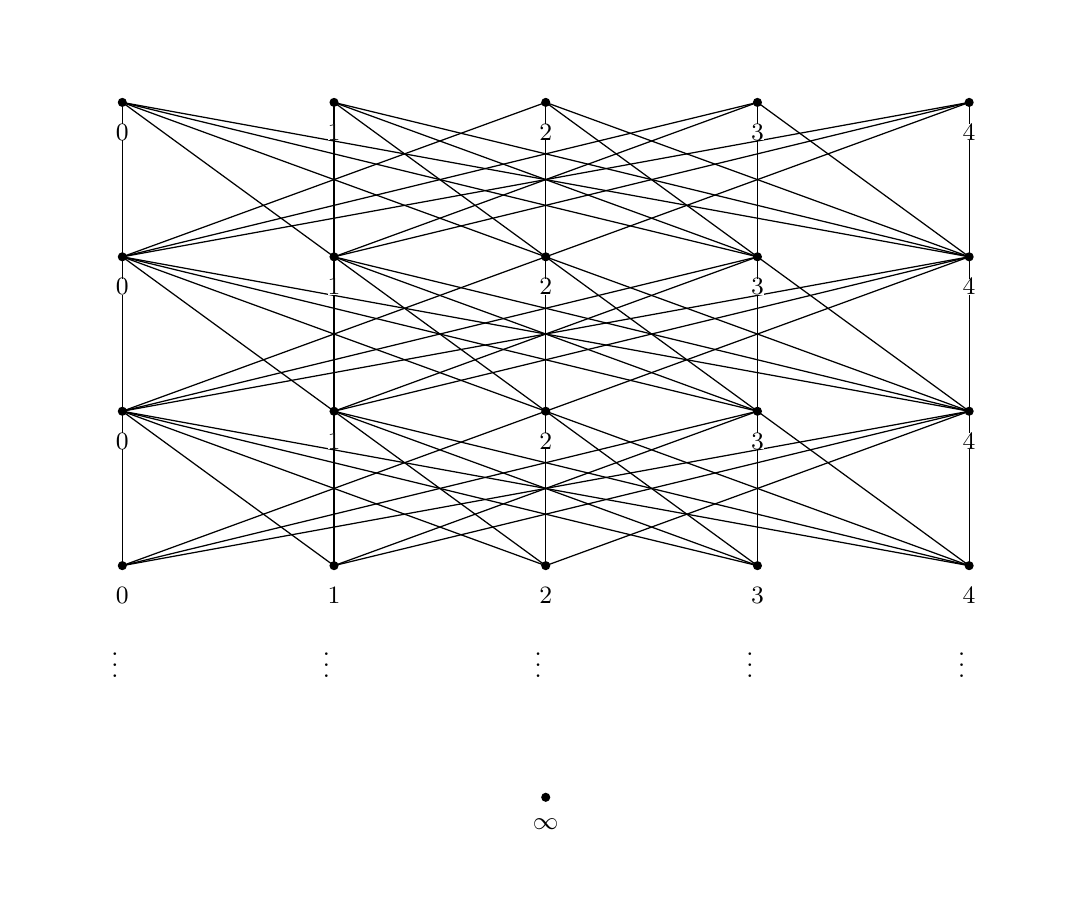
\begin{tikzpicture}[x=.45pt,y=-.45pt,line width=.45pt,line cap=round,font=\fontsize{9}{10}\selectfont]
\path[use as bounding box] (84,22) rectangle (910,710);
\coordinate (nh0v0) at (160,82);
\coordinate (nh0v1) at (330,82);
\coordinate (nh0v2) at (500,82);
\coordinate (nh0v3) at (670,82);
\coordinate (nh0v4) at (840,82);
\coordinate (nh1v0) at (160,206);
\coordinate (nh1v1) at (330,206);
\coordinate (nh1v2) at (500,206);
\coordinate (nh1v3) at (670,206);
\coordinate (nh1v4) at (840,206);
\coordinate (nh2v0) at (160,330);
\coordinate (nh2v1) at (330,330);
\coordinate (nh2v2) at (500,330);
\coordinate (nh2v3) at (670,330);
\coordinate (nh2v4) at (840,330);
\coordinate (nh3v0) at (160,454);
\coordinate (nh3v1) at (330,454);
\coordinate (nh3v2) at (500,454);
\coordinate (nh3v3) at (670,454);
\coordinate (nh3v4) at (840,454);
\coordinate (ninfinity) at (500,640);
\draw (nh1v0) -- (nh0v0);
\draw (nh1v0) -- (nh0v2);
\draw (nh1v0) -- (nh0v3);
\draw (nh1v0) -- (nh0v4);
\draw (nh1v1) -- (nh0v0);
\draw (nh1v1) -- (nh0v1);
\draw (nh1v1) -- (nh0v3);
\draw (nh1v1) -- (nh0v4);
\draw (nh1v2) -- (nh0v0);
\draw (nh1v2) -- (nh0v1);
\draw (nh1v2) -- (nh0v2);
\draw (nh1v2) -- (nh0v4);
\draw (nh1v3) -- (nh0v0);
\draw (nh1v3) -- (nh0v1);
\draw (nh1v3) -- (nh0v2);
\draw (nh1v3) -- (nh0v3);
\draw (nh1v4) -- (nh0v0);
\draw (nh1v4) -- (nh0v1);
\draw (nh1v4) -- (nh0v2);
\draw (nh1v4) -- (nh0v3);
\draw (nh1v4) -- (nh0v4);
\draw (nh2v0) -- (nh1v0);
\draw (nh2v0) -- (nh1v2);
\draw (nh2v0) -- (nh1v3);
\draw (nh2v0) -- (nh1v4);
\draw (nh2v1) -- (nh1v0);
\draw (nh2v1) -- (nh1v1);
\draw (nh2v1) -- (nh1v3);
\draw (nh2v1) -- (nh1v4);
\draw (nh2v2) -- (nh1v0);
\draw (nh2v2) -- (nh1v1);
\draw (nh2v2) -- (nh1v2);
\draw (nh2v2) -- (nh1v4);
\draw (nh2v3) -- (nh1v0);
\draw (nh2v3) -- (nh1v1);
\draw (nh2v3) -- (nh1v2);
\draw (nh2v3) -- (nh1v3);
\draw (nh2v4) -- (nh1v0);
\draw (nh2v4) -- (nh1v1);
\draw (nh2v4) -- (nh1v2);
\draw (nh2v4) -- (nh1v3);
\draw (nh2v4) -- (nh1v4);
\draw (nh3v0) -- (nh2v0);
\draw (nh3v0) -- (nh2v2);
\draw (nh3v0) -- (nh2v3);
\draw (nh3v0) -- (nh2v4);
\draw (nh3v1) -- (nh2v0);
\draw (nh3v1) -- (nh2v1);
\draw (nh3v1) -- (nh2v3);
\draw (nh3v1) -- (nh2v4);
\draw (nh3v2) -- (nh2v0);
\draw (nh3v2) -- (nh2v1);
\draw (nh3v2) -- (nh2v2);
\draw (nh3v2) -- (nh2v4);
\draw (nh3v3) -- (nh2v0);
\draw (nh3v3) -- (nh2v1);
\draw (nh3v3) -- (nh2v2);
\draw (nh3v3) -- (nh2v3);
\draw (nh3v4) -- (nh2v0);
\draw (nh3v4) -- (nh2v1);
\draw (nh3v4) -- (nh2v2);
\draw (nh3v4) -- (nh2v3);
\draw (nh3v4) -- (nh2v4);
\node at (154,527) {$\vdots$};
\node at (324,527) {$\vdots$};
\node at (494,527) {$\vdots$};
\node at (664,527) {$\vdots$};
\node at (834,527) {$\vdots$};
\fill (nh0v0) circle[radius=1.65pt];
\node[anchor=north,inner sep=0pt,fill=white] at (160,99) {$0$};
\fill (nh0v1) circle[radius=1.65pt];
\node[anchor=north,inner sep=0pt,fill=white] at (330,99) {$1$};
\fill (nh0v2) circle[radius=1.65pt];
\node[anchor=north,inner sep=0pt,fill=white] at (500,99) {$2$};
\fill (nh0v3) circle[radius=1.65pt];
\node[anchor=north,inner sep=0pt,fill=white] at (670,99) {$3$};
\fill (nh0v4) circle[radius=1.65pt];
\node[anchor=north,inner sep=0pt,fill=white] at (840,99) {$4$};
\fill (nh1v0) circle[radius=1.65pt];
\node[anchor=north,inner sep=0pt,fill=white] at (160,223) {$0$};
\fill (nh1v1) circle[radius=1.65pt];
\node[anchor=north,inner sep=0pt,fill=white] at (330,223) {$1$};
\fill (nh1v2) circle[radius=1.65pt];
\node[anchor=north,inner sep=0pt,fill=white] at (500,223) {$2$};
\fill (nh1v3) circle[radius=1.65pt];
\node[anchor=north,inner sep=0pt,fill=white] at (670,223) {$3$};
\fill (nh1v4) circle[radius=1.65pt];
\node[anchor=north,inner sep=0pt,fill=white] at (840,223) {$4$};
\fill (nh2v0) circle[radius=1.65pt];
\node[anchor=north,inner sep=0pt,fill=white] at (160,347) {$0$};
\fill (nh2v1) circle[radius=1.65pt];
\node[anchor=north,inner sep=0pt,fill=white] at (330,347) {$1$};
\fill (nh2v2) circle[radius=1.65pt];
\node[anchor=north,inner sep=0pt,fill=white] at (500,347) {$2$};
\fill (nh2v3) circle[radius=1.65pt];
\node[anchor=north,inner sep=0pt,fill=white] at (670,347) {$3$};
\fill (nh2v4) circle[radius=1.65pt];
\node[anchor=north,inner sep=0pt,fill=white] at (840,347) {$4$};
\fill (nh3v0) circle[radius=1.65pt];
\node[anchor=north,inner sep=0pt,fill=white] at (160,471) {$0$};
\fill (nh3v1) circle[radius=1.65pt];
\node[anchor=north,inner sep=0pt,fill=white] at (330,471) {$1$};
\fill (nh3v2) circle[radius=1.65pt];
\node[anchor=north,inner sep=0pt,fill=white] at (500,471) {$2$};
\fill (nh3v3) circle[radius=1.65pt];
\node[anchor=north,inner sep=0pt,fill=white] at (670,471) {$3$};
\fill (nh3v4) circle[radius=1.65pt];
\node[anchor=north,inner sep=0pt,fill=white] at (840,471) {$4$};
\fill (ninfinity) circle[radius=1.65pt];
\node[anchor=north,inner sep=0pt,fill=white] at (500,657) {$\infty$};
\end{tikzpicture}
\end{document}
